 \subsubsection{UC10 - Gestione veicoli}
  \begin{figure}[H]
 	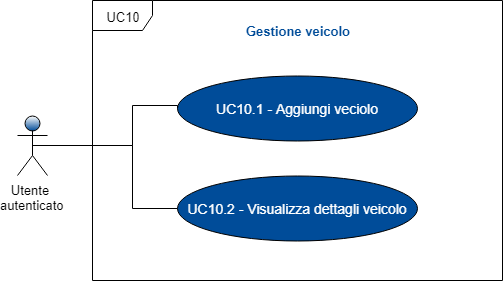
\includegraphics[width=10cm]{res/images/UC10Gestioneveicolo.png}
 	\centering
 	\caption{UC10 - Gestione veicoli}
 \end{figure}
 \begin{itemize}
 	\item \textbf{Attori Primari}: utente autenticato;
 	\item \textbf{Descrizione}: l'utente ha una panoramica dei veicoli che ha inserito visualizzando solo poche cose riguardanti il mezzo e ha la possibilità di:
 	\begin{itemize}
 		\item aggiungere un veicolo [UC10.1];
 		\item visualizzare i dettagli del veicolo [UC10.2];
 		\item aggiungere disponibilità del veicolo [UC10.3];
 		\item rimuovere un veicolo [UC10.4].
 	\end{itemize}
 	\item \textbf{Precondizione}: l'utente accede al fragment\glosp per la gestione dei veicoli;
 	\item \textbf{Postcondizione}: l'utente visualizza le informazioni relative ai propri veicoli, con le eventuali operazioni disponibili su ognuno di essi.
 \end{itemize}
 \subsubsection{UC10.1 - Aggiungi veicolo}
 \begin{itemize}
 	\item \textbf{Attori Primari}: utente autenticato;
 	\item \textbf{Descrizione}: l'utente può aggiungere un mezzo di trasporto al proprio parco macchine;
 	\item \textbf{Scenario principale}: l'utente aggiunge un veicolo compilando gli appositi campi obbligatori, ovvero:
 	\begin{itemize}
 		\item inserimento immagine veicolo [UC10.1.1];
 		\item inserimento marca veicolo [UC10.1.2];
 		\item inserimento modello veicolo [UC10.1.3];
 		\item inserimento anno d'immatricolazione veicolo [UC10.1.4];
 		\item inserimento posizione veicolo [UC10.1.5].
 	\end{itemize}
 	e successivamente salverà il nuovo veicolo confermando i campi appena inseriti;
 	\item \textbf{Precondizione}: l'utente ha inserito correttamente tutti i campi necessari;
 	\item \textbf{Postcondizione}: il nuovo veicolo viene aggiunto ai veicoli posseduti.
 \end{itemize}
\begin{figure}[H]
	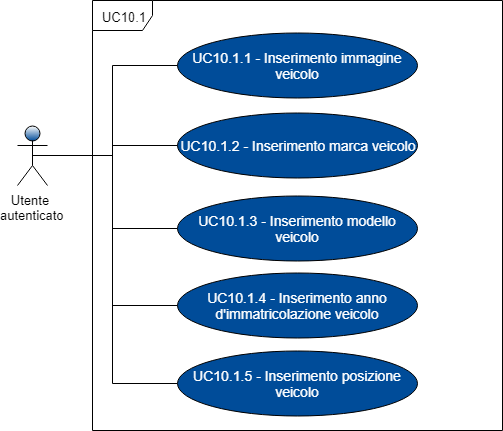
\includegraphics[width=10cm]{res/images/UC10-1Aggiungiveicolo.png}
	\centering
	\caption{UC10.1 - Aggiungi veicolo}
\end{figure}
\subsubsection{UC10.1.1 - Inserimento immagine veicolo}
\begin{itemize}
	\item \textbf{Attori Primari}: utente autenticato;
	\item \textbf{Descrizione}: al fine di portare a termine il processo di inserimento di un nuovo veicolo l'utente deve inserire un'immagine del proprio mezzo, campo ritenuto obbligatorio; 
	\item \textbf{Scenario principale}: l'utente preme il pulsante relativo all'inserimento dell'immagine del veicolo;	
	\item \textbf{Precondizione}: l'applicazione ha reso disponibile il bottone per l'inserimento dell'immagine del veicolo;
	\item \textbf{Postcondizione}: l'utente ha inserito correttamente l'immagine del veicolo.
\end{itemize}
\subsubsection{UC10.1.2 - Inserimento marca veicolo}
\begin{itemize}
	\item \textbf{Attori Primari}: utente autenticato;
	\item \textbf{Descrizione}: al fine di portare a termine il processo di inserimento di un nuovo veicolo l'utente deve inserire la marca, campo ritenuto obbligatorio;
	\item \textbf{Scenario principale}: l'utente compila il campo relativo alla marca del veicolo;	
	\item \textbf{Precondizione}: l'applicazione ha reso disponibile il campo per l'inserimento della marca del veicolo;
	\item \textbf{Postcondizione}: l'utente ha compilato il campo con la marca.	
\end{itemize}

\subsubsection{UC10.1.3 - Inserimento modello veicolo}
\begin{itemize}
	\item \textbf{Attori Primari}: utente autenticato;
	\item \textbf{Descrizione}: al fine di portare a termine il processo di inserimento di un nuovo veicolo l'utente deve inserire il modello, campo ritenuto obbligatorio;
	\item \textbf{Scenario principale}: l'utente compila il campo relativo alla marca del veicolo;	
	\item \textbf{Precondizione}: l'applicazione ha reso disponibile il campo per l'inserimento il modello del veicolo;
	\item \textbf{Postcondizione}: l'utente ha compilato il campo con il modello.	
\end{itemize}
\subsubsection{UC10.1.4 - Inserimento anno d'immatricolazione veicolo}
\begin{itemize}
	\item \textbf{Attori Primari}: utente autenticato;
	\item \textbf{Descrizione}: al fine di portare a termine il processo di inserimento di un nuovo veicolo l'utente deve inserire l'anno di immatricolazione, campo ritenuto obbligatorio;
	\item \textbf{Scenario principale}: l'utente compila il campo relativo all'anno d'immatricolazione del veicolo;	
	\item \textbf{Precondizione}: l'applicazione ha reso disponibile il campo per l'inserimento dell'anno d'immatricolazione del veicolo;
	\item \textbf{Postcondizione}: l'utente ha compilato il campo con l'anno d'immatricolazione.	
\end{itemize}
\subsubsection{UC10.1.5 - Inserimento posizione veicolo}
\begin{itemize}
	\item \textbf{Attori Primari}: utente autenticato;
	\item \textbf{Descrizione}: al fine di portare a termine il processo di inserimento di un nuovo veicolo l'utente deve inserire la posizione del proprio veicolo campo ritenuto obbligatorio;
	\item \textbf{Scenario principale}: l'utente compila il campo relativo alla posizione del veicolo;	
	\item \textbf{Precondizione}: l'applicazione ha reso disponibile il campo per l'inserimento della posizione del veicolo;
	\item \textbf{Postcondizione}: l'utente ha compilato il campo con la posizione del veicolo.	
\end{itemize}
\subsubsection{UC10.2 - Visualizza dettagli veicolo}
\begin{itemize}
	\item \textbf{Attori Primari}: utente autenticato;
	\item \textbf{Descrizione}: l'utente autenticato, per ogni veicolo, può visualizzare in dettaglio le seguenti informazioni:
	\begin{itemize}
		\item marca;
		\item modello;
		\item anno di immatricolazione;
		\item rating.
	\end{itemize}
	e ha la possibilità di aggiungere disponibilità del veicolo [UC10.3] o rimuoverlo [UC10.4];
	\item \textbf{Scenario principale}: l'utente visualizza i dati di dettaglio del veicolo;
	\item \textbf{Precondizione}: l'utente autenticato visualizza i dettagli del veicolo;
	\item \textbf{Postcondizione}: l'utente autenticato ha visualizzato i dettagli del veicolo.
\end{itemize}
\subsubsection{UC10.3 - Aggiungi disponibilità}
\begin{figure}[H]
	%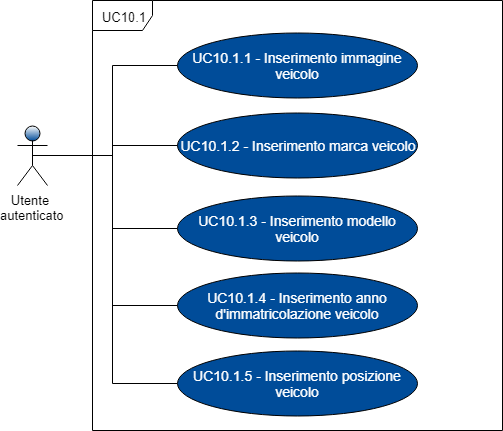
\includegraphics[width=10cm]{res/images/UC10-1Aggiungiveicolo.png}
	\centering
	\caption{UC10.3 - Aggiungi disponibilità}
\end{figure}
\begin{itemize}
	\item \textbf{Attori Primari}: utente autenticato;
	\item \textbf{Descrizione}: l'utente può inserire la disponibilità in cui mette a disposizione il proprio veicolo inserendo data e ora;
	\item \textbf{Scenario principale}: l'utente, dopo aver selezionato il veicolo da visualizzare, può aggiungere la disponibilità del veicolo inserendo:
	\begin{itemize}
		\item data prenotazione [UC10.3.1];
		\item ora di inizio [UC10.3.2];
		\item ora di fine [UC10.3.3].
	\end{itemize}
	e successivamente confermando l'aggiunta della disponibilità, l'utente viene rimandato nell'area di \textit{Gestione veicolo};
	\item \textbf{Scenario alternativo}: l'utente, dopo aver selezionato il veicolo da visualizzare, può decidere di ripetere la disponibilità del veicolo. In questo caso l'utente inserisce:
	\begin{itemize}
		\item ora di inizio [10.3.2];
		\item ora di fine [10.3.3];
		\item ripetizione per quali giorni [10.3.4];
		\item ripetizione per quanto tempo [10.3.5].
	\end{itemize}
	e successivamente confermando l'aggiunta della disponibilità, l'utente viene rimandato nell'area di \textit{Gestione veicolo};
	\item \textbf{Precondizione}: l'applicazione mostra all'utente i propri veicoli e ne permette la selezione;
	\item \textbf{Postcondizione}: viene aggiunta la disponibilità al veicolo selezionato.
\end{itemize}
\subsubsection{UC10.3.1 - Inserimento data prenotazione}
\begin{itemize}
	\item \textbf{Attori Primari}: utente autenticato;
	\item \textbf{Descrizione}: al fine di portare a termine il processo di aggiunta della disponibilità al veicolo, l'utente deve inserire la data di prenotazione. Visualizzerà un calendario dove potrà selezionare un giorno del mese che preferisce;
	\item \textbf{Scenario principale}: l'utente compila il campo relativo alla data di prenotazione;	
	\item \textbf{Precondizione}: l'applicazione ha reso disponibile il campo per l'inserimento della data di prenotazione;
	\item \textbf{Postcondizione}: l'utente ha compilato il campo con la data di prenotazione.	
\end{itemize}
\subsubsection{UC10.3.2 - Inserimento ora di inizio}
\begin{itemize}
	\item \textbf{Attori Primari}: utente autenticato;
	\item \textbf{Descrizione}: al fine di portare a termine il processo di aggiunta della disponibilità al veicolo, l'utente deve inserire l'ora di inizio in cui un usufruente può prenotare l'auto. L'orario viene mostrato in fasce orarie da 15 minuti;
	\item \textbf{Scenario principale}: l'utente compila il campo relativo all'ora di inizio;	
	\item \textbf{Precondizione}: l'applicazione ha reso disponibile il campo per l'inserimento dell'ora di inizio;
	\item \textbf{Postcondizione}: l'utente ha compilato il campo con l'ora di inizio.	
\end{itemize}
\subsubsection{UC10.3.3 - Inserimento ora di fine}
\begin{itemize}
	\item \textbf{Attori Primari}: utente autenticato;
	\item \textbf{Descrizione}: al fine di portare a termine il processo di aggiunta della disponibilità al veicolo, l'utente deve inserire l'ora di fine in cui un usufruente può prenotare l'auto. L'orario viene mostrato in fasce orarie da 15 minuti;
	\item \textbf{Scenario principale}: l'utente compila il campo relativo all'ora di fine;	
	\item \textbf{Precondizione}: l'applicazione ha reso disponibile il campo per l'inserimento dell'ora di fine;
	\item \textbf{Postcondizione}: l'utente ha compilato il campo con l'ora di fine.	
\end{itemize}
\subsubsection{UC10.3.4 - Inserimento ripetizione giorni della settimana}
\begin{itemize}
	\item \textbf{Attori Primari}: utente autenticato;
	\item \textbf{Descrizione}: al fine di portare a termine il processo di aggiunta della disponibilità al veicolo, l'utente deve inserire i giorni della settimana in cui vuole che il veicolo sia disponibile;
	\item \textbf{Scenario principale}: l'utente compila il campo relativo all'inserimento dei giorni della settimana in cui ripetere la disponibilità;	
	\item \textbf{Precondizione}: l'applicazione ha reso disponibile il campo per l'inserimento dei giorni della settimana in cui rendere disponibile il veicolo;
	\item \textbf{Postcondizione}: l'utente ha compilato il campo con i giorni della settimana in cui vuole ripetere la disponibilità.	
\end{itemize}
\subsubsection{UC10.3.5 - Inserimento ripetizione quantità di tempo}
\begin{itemize}
	\item \textbf{Attori Primari}: utente autenticato;
	\item \textbf{Descrizione}: al fine di portare a termine il processo di aggiunta della disponibilità al veicolo, l'utente deve inserire la quantità di tempo in cui la disponibilità del veicolo deve essere ripetuta;
	\item \textbf{Scenario principale}: l'utente compila il campo relativo all'inserimento della quantità di tempo in cui la disponibilità del veicolo deve essere ripetuta;	
	\item \textbf{Precondizione}: l'applicazione ha reso disponibile il campo per l'inserimento della quantità di tempo in cui la disponibilità del veicolo deve essere ripetuta;
	\item \textbf{Postcondizione}: l'utente ha compilato il campo con la quantità di tempo in cui la disponibilità del veicolo deve essere ripetuta.	
\end{itemize}
\subsubsection{UC10.4 - Rimuovi veicolo}
\begin{itemize}
	\item \textbf{Attori Primari}: utente autenticato;
	\item \textbf{Descrizione}: l'utente può rimuovere un mezzo di trasporto dal proprio parco macchine;
	\item \textbf{Scenario principale}: l'utente, dopo aver selezionato il veicolo da visualizzare, può rimuoverlo dal proprio parco macchine attraverso l'apposito pulsante;
	\item \textbf{Precondizione}: l'applicazione mostra all'utente i propri veicoli e ne permette la selezione;
	\item \textbf{Postcondizione}: il veicolo selezionato viene rimosso dal parco macchine.
\end{itemize}